% journal of hydrology
% !TEX TS-program = pdflatex
% !TEX encoding = UTF-8 Unicode

% This is a simple template for a LaTeX document using the "article" class.
% See "book", "report", "letter" for other types of document.

\documentclass[11pt]{article} % use larger type; default would be 10pt

\usepackage[utf8]{inputenc} % set input encoding (not needed with XeLaTeX)

%%% Examples of Article customizations
% These packages are optional, depending whether you want the features they provide.
% See the LaTeX Companion or other references for full information.

%%% PAGE DIMENSIONS
\usepackage{geometry} % to change the page dimensions
\geometry{a4paper} % or letterpaper (US) or a5paper or....
% \geometry{margin=2in} % for example, change the margins to 2 inches all round
% \geometry{landscape} % set up the page for landscape
%   read geometry.pdf for detailed page layout information

\usepackage{graphicx} % support the \includegraphics command and options

% \usepackage[parfill]{parskip} % Activate to begin paragraphs with an empty line rather than an indent

%%% PACKAGES
\usepackage{url}
\usepackage{hyperref}
\usepackage{listings}
\usepackage{booktabs} % for much better looking tables
\usepackage{array} % for better arrays (eg matrices) in maths
\usepackage{paralist} % very flexible & customisable lists (eg. enumerate/itemize, etc.)
\usepackage{verbatim} % adds environment for commenting out blocks of text & 
%for better verbatim
%\usepackage{amsmath}
\usepackage{amsmath,amssymb}
\DeclareMathOperator{\E}{\mathbb{E}}

\usepackage{natbib}
\bibliographystyle{abbrvnat}
\setcitestyle{authoryear,open={((},close={))}}

\usepackage{subfigure}
%\usepackage{pageslts}

%\usepackage{subfig} % make it possible to include more than one captioned 
%%figure/table in a single float
% These packages are all incorporated in the memoir class to one degree or another...

%%% HEADERS & FOOTERS
\usepackage{fancyhdr} % This should be set AFTER setting up the page geometry
\pagestyle{fancy} % options: empty , plain , fancy
%\renewcommand{\headrulewidth}{0pt} % customise the layout...
%\lhead{}\chead{}\rhead{}
\lfoot{}\cfoot{\thepage}\rfoot{}
%\lfoot{}\cfoot{Page \thepage\ (\theCurrentPage) of 
%\lastpageref{LastPages}}\rfoot{}

%%% SECTION TITLE APPEARANCE
\usepackage{sectsty}
\allsectionsfont{\sffamily\mdseries\upshape} % (See the fntguide.pdf for font help)
% (This matches ConTeXt defaults)

%%% ToC (table of contents) APPEARANCE
\usepackage[nottoc,notlof,notlot]{tocbibind} % Put the bibliography in the ToC
\usepackage[titles,subfigure]{tocloft} % Alter the style of the Table of Contents
\renewcommand{\cftsecfont}{\rmfamily\mdseries\upshape}
\renewcommand{\cftsecpagefont}{\rmfamily\mdseries\upshape} % No bold!

%%% END Article customizations

%%% The "real" document content comes below...

\title{Final Report (Draft): \\
Image Analysis using Artificial Intelligence to
Quantify the Number and Density of Mussels in Lake Erie and Ontario}

\author{Angus Galloway}
%\date{} % Activate to display a given date or no date (if empty),
         % otherwise the current date is printed
         
\pagenumbering{roman}         

\begin{document}

\maketitle

\thispagestyle{empty}

\vspace{5cm}

\begin{centering}

Report prepared for:

\vspace{1cm}

Dominique Brunet \\ 
Environment Canada \\ 
867 Lakeshore Rd \\
Burlington, ON \\
L7S 1A1 

\end{centering}

\clearpage

% an introduction, a technical discussion of the steps taken, the rationale for
% the various design choices made and parameters selected for the training of
% the computer vision model, a technical discussion summarizing the
% strengths and limitations of the computer vision model and its robustness to 
% change to change of image resolution, viewing angle and other relevant
% factors, a discussion detailing how data acquisition methods can be improved
% in future surveys, and conclusions and include, as applicable, supporting
% graphs, tables and figures.

\setcounter{page}{1}

\section*{Executive Summary}
% 250 words or less

Goes here

\clearpage

\tableofcontents

\clearpage

\section*{Abbreviations}

\begin{description}
\item[ML] machine learning
\item[DL] deep learning
\item[DNN] deep neural network
\item[CNN] convolutional neural network
\item[FCN] fully convolutional neural network
\item[CE] Cross entropy
\item[SGD] stochastic gradient descent
\item[IoU] intersection over union
\item[mIoU] mean IoU
\item[TP] true positive
\item[w.r.t.] with respect to
\end{description}

\clearpage

\pagenumbering{arabic}
\setcounter{page}{1}

\section{Introduction}

The task of predicting mussel biomass, count, and percent coverage was cast as
that of~\emph{semantic segmentation} in machine learning. This means that a 
categorical prediction is assigned to each pixel in an image, where the
categories are assumed to have some semantic meaning, for example 
``pedestrian'', ``road'', or ``vehicle''.

\section{Data Preparation}

\section{Machine Learning Methodology}

The practice of machine learning involves the selection, or search for ``good'' 
meta-parameters. The prefix ``meta'' is used to distinguish the parameters of
the learning algorithm -- generally set by the practitioner -- from those of the
model, which are to be learned.\footnote{Meta-parameters are often called
hyper-parameters, but the latter term is reserved for parameters of 
probability distributions.}

Relevant meta-parameters include the step size or ``learning rate'' of gradient
descent (GD), and the mini-batch size, which is what distinguishes stochastic
gradient descent (SGD) from full-batch GD. 

Optional meta-parameters include L2 regularization, aka ``weight decay'',
which penalizes the squared $\ell_2$-norm of all parameters of the model.

Denote the neural network parameters at time step $t$ by $\theta_t$. The update
equation which determines the parameters at the next time step, $\theta_{t + 
1}$, is then:

\begin{equation} \label{eq:sgd}
\theta_{t + 1} = \theta_t + \eta \nabla_{\theta} \mathop{\mathbb{E}}_{x,y \sim 
X, Y} \big[ \mathcal{L}(y, \hat{y}) \big]
\end{equation}

The loss function $\mathcal{L}$ has as its arguments the input $x$, ground
truth labels $y$, and model predictions $\hat{y}$. Assume access to a dataset 
of $N$ samples (technically a sequence not a set) of pairs 
$\{ (x_i, y_i)\}_{i=1}^{N} $.

\subsection{Learning Rate Selection}

The learning rate, $\eta$ in Eq.~\eqref{eq:sgd}, controls the magnitude of the 
updates to the parameters at each update step. There is significant theory on
the optimal selection of learning rates in the case where the loss is a convex
function of the parameters, but less so when the loss is non-convex w.r.t.~the
parameters, as is the case in deep learning. Here, researchers often perform
simulations to determine the best learning rate on the basis of validation 
accuracy.

Nevertheless, some general comments can be made on the topic of learning rate 
selection in DL: 

\begin{enumerate}
\item a larger learning rate generally reduces the loss more quickly than a
smaller learning rate allowing one to see results more quickly, but, \dots
\item a larger learning rate may make training unstable
\item a larger learning rate -- for a fixed mini-batch size -- can be said to
be noisier than a smaller learning rate. Such noise tends to be helpful for 
promoting generalization, e.g., wide minima argument, however if the gradient 
is too noisy then the gradient signal-to-noise ratio may be too low thus 
slowing learning.
\item on the regularization effect of large initial learning rate.
\end{enumerate}

\subsection{Mini-Batch Size Selection}

Generally, there is a strong interplay between the batch size and the learning
rate. For training efficiency, one generally prefers the largest batch size
without overflowing available GPU memory.

Too large a batch size behaves similarly as too small a learning rate, thus may 
converge to a ``sharper'' minimum of the loss landscape. Conversely, too small 
a batch and the variance of the expectation in Eq.~\eqref{eq:sgd} will be too 
high.

\subsection{Segmentation Model Architectures}

Several segmentation architectures based on deep neural networks were
considered: 

\begin{description}
\item[FCN] Fully convolutional networks (FCN) were proposed 
by~\cite{long2015fully} \dots

\item[U-Net] Was originally proposed by~\cite{ronneberger2015unet} for 
biomedical image segmentation, where sharp edge boundaries, for example between 
affected and unaffected skin lessions are important. This architecture has 
since been successfully applied in many natural image domains unrelated to 
medical imaging. 
The model takes its name from its ``U'' shaped network diagram whereby the
input is encoded into a progressively smaller representation which reaches a 
bottleneck at the bottom of the ``U'', which is then gradually upsampled to the 
original image size while features from earlier encodings are concatenated to 
the decoded representations at each layer for spatial consistency.

\item[DeepLab] desc

\item[CRF] The conditional random field~\cite{krahenbuhl2011efficient} is not
itself a segmentation architecture, but a graphical model that is commonly used
for~\emph{structured prediction} tasks, and post-processing segmentation
predictions in particular.

\end{description}

\subsection{Evaluation Criteria}

Semantic segmentation performance is generally assessed in terms of the
intersection between predictions and the ground truth segmentation mask -- the
true positives -- divided by the union of the predictions and the ground truth, 
which includes both false negatives and false positives. This quantity is
referred to as the intersection-over-union (IoU), or mIoU after taking the
mean over samples in a dataset. This metric addresses a limitation of reporting 
pixelwise accuracy, since most datasets are dominated by background pixels,
thus a high accuracy could be obtained by a constant classifier that simply
predicts ``background''. Conversely, the binary IoU is formally defined as:

\begin{equation}
\frac{TP}{FN + TP + FP}
\end{equation}

Despite its widespread use, the binary mIoU metric has some limitations:

\begin{enumerate}
\item If legitimate images contain~\emph{none} of the foreground classes, i.e.,
the true label is $100\%$ background, the numerator ``TP'' is undefined and an
IoU score of 0 is assigned to a ``true negative'' prediction.

\item If the foreground pixel area varies significantly, IoU 
scores may be less comparable between images. For example, an image with $1\%$
\texttt{mussel} pixels in which $90\%$ are predicted correctly would be assigned
an equal weight w.r.t.~the sample mean as an image with $50\%$~\texttt{mussel}
of which only $50\%$ are identified as such. In this scenario, the sample with
$1\%$~\texttt{mussel} inflates the mIoU score.
\end{enumerate}

In light of these limitations, several variants of mIoU have been proposed to 
incorporate various weighting schemes.

\subsection{Data Augmentation and Pre-Processing}

\begin{enumerate}

\item Randomly flip images horizontally and vertically.

\item Normalize pixels from [0, 1] to [-1, 1].

\end{enumerate}

\section{Experiments}

The underwater dataset is referred to as ``In-Situ''.

\subsection{Mussel Biomass Prediction from Ground Truth Segmentation}

In this section we assess the quality of the obtained segmentation labels and
characterize the noise inherent in relating the mussel biomass to those mussels
identifiable by human eye.

\begin{figure}
\centering
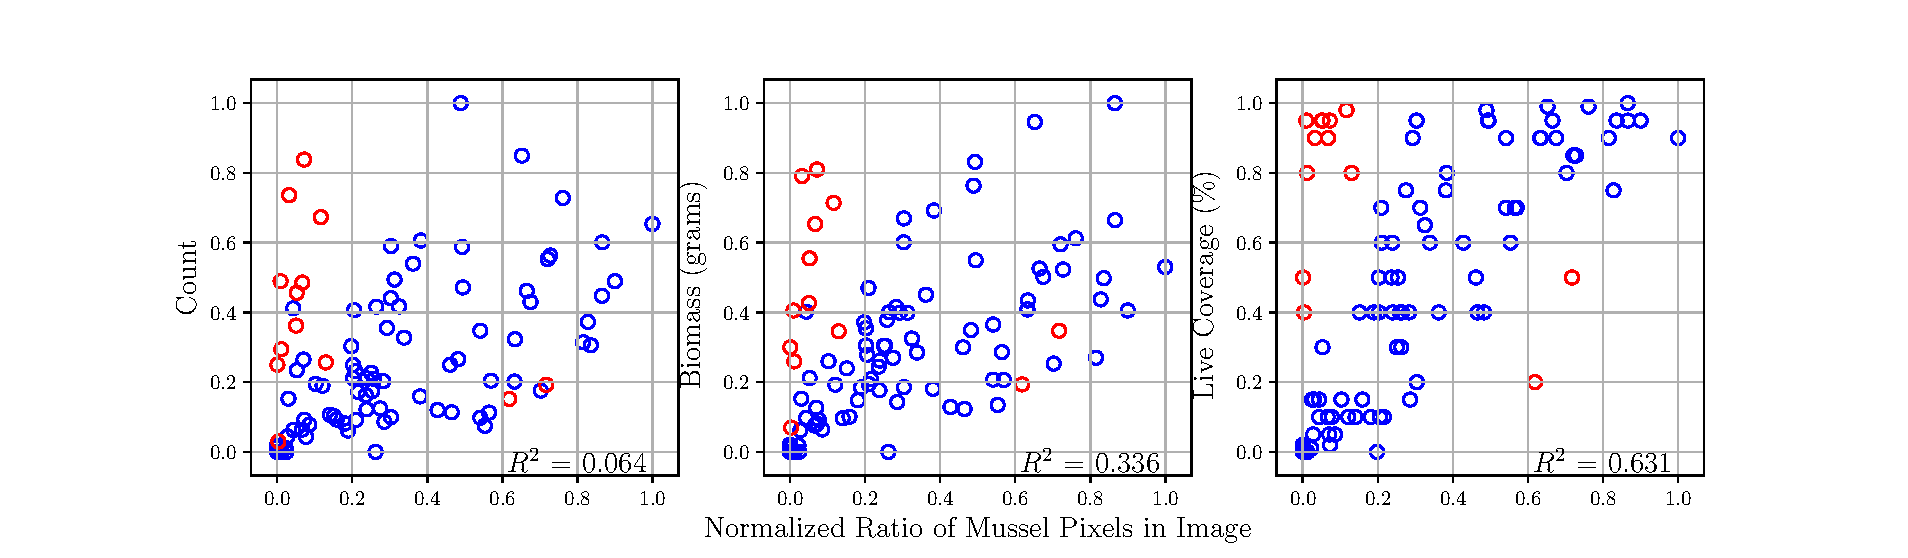
\includegraphics[width=0.9\linewidth]{img/Train-all-109-annotate-outliers}
\caption{Relationship between mussel count, biomass, and diver estimated live
mussel coverage versus pixels assigned to mussel class in ground truth
segmentation labels for GLNI training data ($N=109$). Note that because only 
those mussels that could be clearly identified as such were labeled, an upper 
triangular effect is observed where some images have few labeled mussels, 
but high biomass (e.g., due to occlusion from~\emph{Cladophora}). Removing 9 
such outliers (shown in red) increases the $R^2$ value three fold from $\approx
0.2$ to $0.63$. All ``outliers'' were intentionally under labeled due to
considerable occlusion by Cladophora, or a lack of illumination.}
\label{fig:train-biomass-from-labels}
\end{figure}


\subsection{Training and Testing on In-Situ Dataset}

plot showing IoU along with CE loss.


\subsection{Training and Testing on Lab Dataset}

See Figure~\ref{fig:lab-to-lab-biomass-from-pixels}.

\newcommand{\labtolab}{./img/lab_to_lab/}

\begin{figure}
\centering
\subfigure[]{
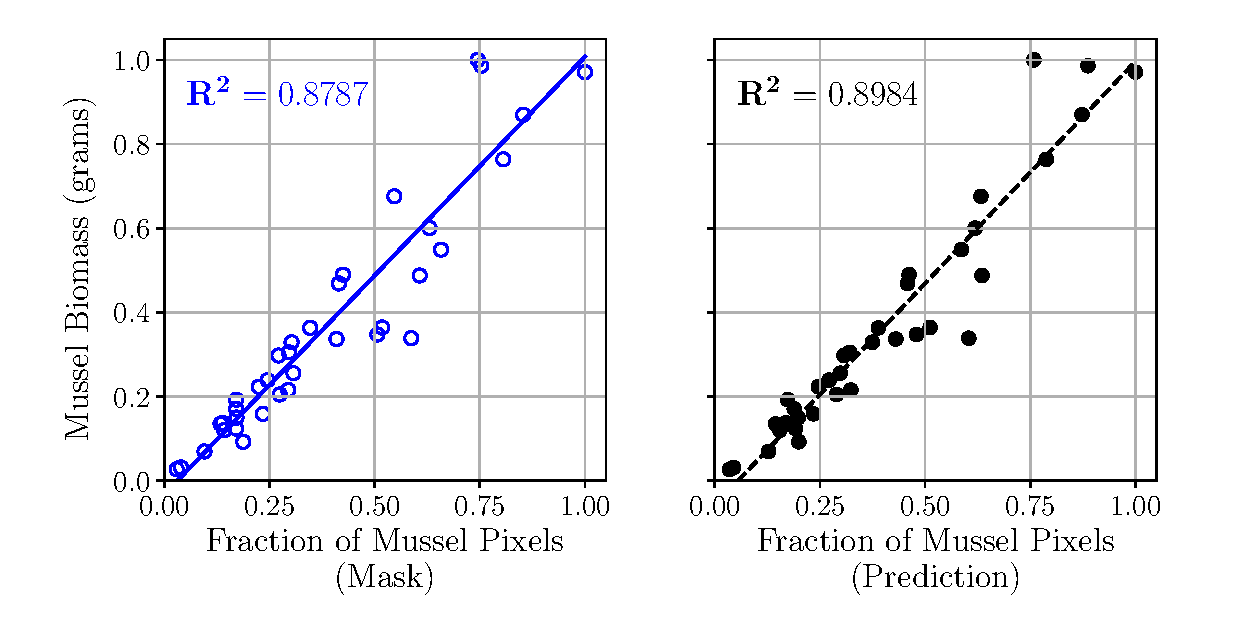
\includegraphics[width=0.9\linewidth]{\labtolab/lab_predict_biomass_from_pixels_no_cameraval_100-val_100__fcn8slim_lr1e-03_wd5e-04_bs32_ep50_seed1_epoch40.eps}
\label{sub:lab-biomass-default}}
\subfigure[]{
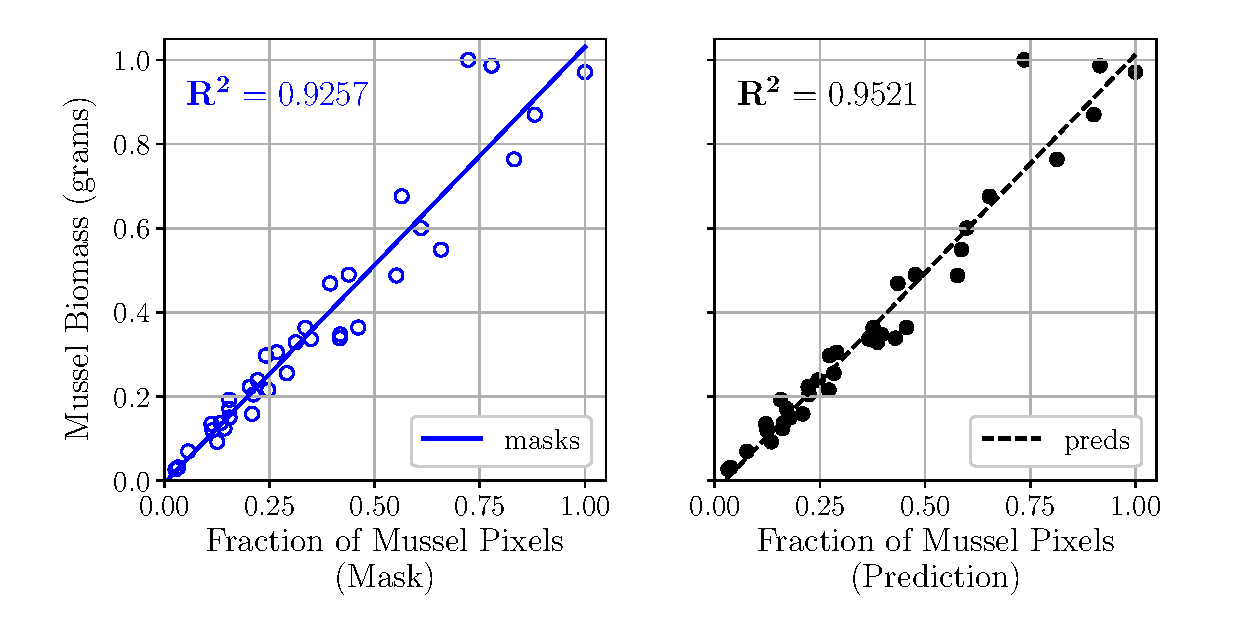
\includegraphics[width=0.9\linewidth]{\labtolab/lab_predict_biomass_from_pixelsval_100-val_100__fcn8slim_lr1e-03_wd5e-04_bs32_ep50_seed1_epoch40.eps}
\label{sub:lab-biomass-camera}}
\caption{Relationship between mussel biomass in grams and fraction of pixels in 
image mask (left column) or prediction (right column) assigned to mussel class.
Plot~\subref{sub:lab-biomass-default} is based on raw pixel count in images, 
while~\subref{sub:lab-biomass-camera} adjusts the number of pixels by the
product of the vertical and horizontal squares in the frame divided by the 
total number of squares ($16 \times 25$). The $R^2$ score, or proportion of
variance in biomass accounted for by mussel pixels is annotated in each plot.}
\label{fig:lab-to-lab-biomass-from-pixels}
\end{figure}

\begin{figure}
\centering
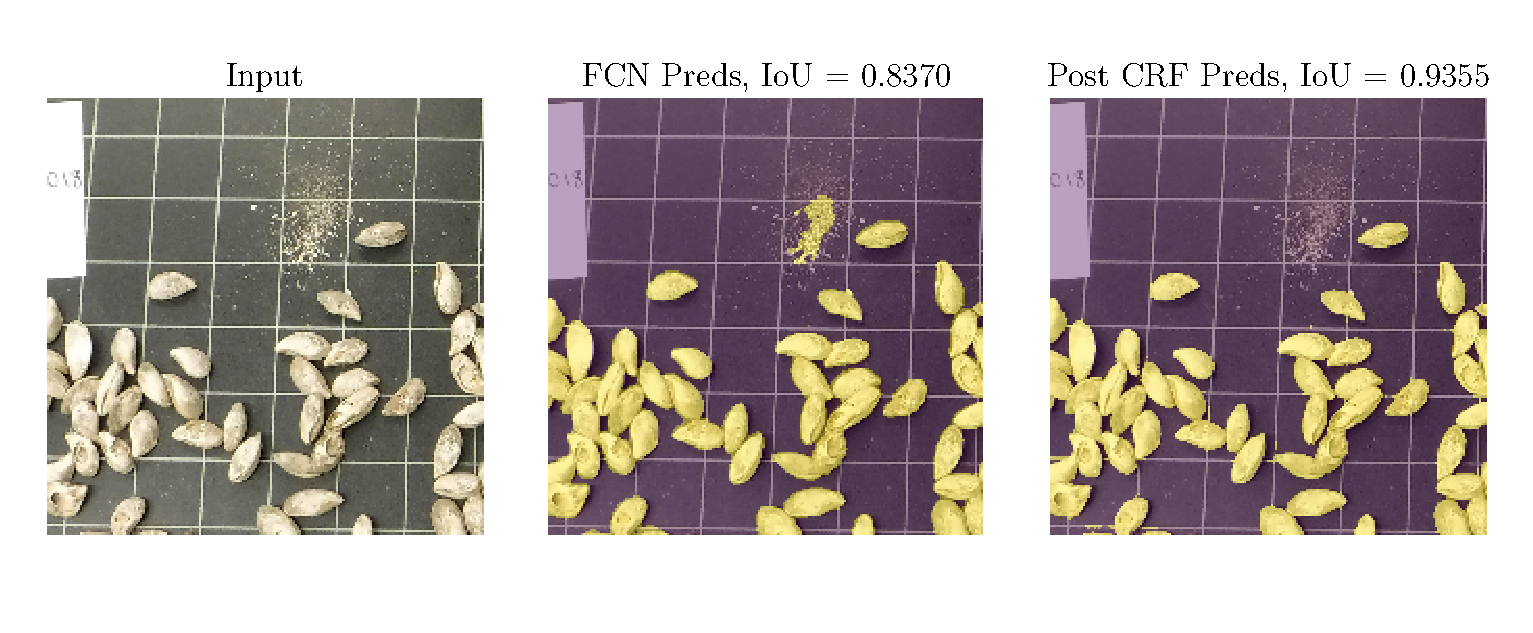
\includegraphics[width=0.9\linewidth]{\labtolab/val_100-val_100__Lab_3796-1_2018-08-13_image-1_patch_width1000_crf__fcn8slim_lr1e-03_wd5e-04_bs32_ep50_seed1_epoch40.eps}
\caption{Sample image patch and predictions with IoU score. Post processing 
by CRF improves IoU by 10\% absolute, primarily by eliminating the FP
predictions associated with the debris.}
\label{fig:lab-to-lab-sample}
\end{figure}


\subsection{Zero-Shot Generalization From In-Situ to Lab Dataset}

Figure~\ref{fig:zero-shot-situ-lab} shows model predictions that arise from
training on underwater data and evaluated on an unseen distribution of Lab
images. The generalization problem is difficult because mussels tend to sit in a
vertical orientation in the wild, with the dark gap between the two shell
halves acting as a primary visual basis for identification by human eye. 
Further, mussels tend to be darker underwater due to reduced illumination, or
from being covered with a fine layer of sediment. Conversely, Lab images are 
well illuminated and all mussels lie on their side. 

These qualitative differences between the two distributions are 
reflected in Figure~\ref{fig:zero-shot-situ-lab}. It appears that the brighter 
mussels -- which have a similar white colour as the unlabeled empty shells
underwater -- are the most prominent false positives, while the darker more 
textured area of the mussle shells are identified correctly.

\newcommand{\zshot}{./img/situ_to_lab/}

\begin{figure}
\centering
\subfigure{
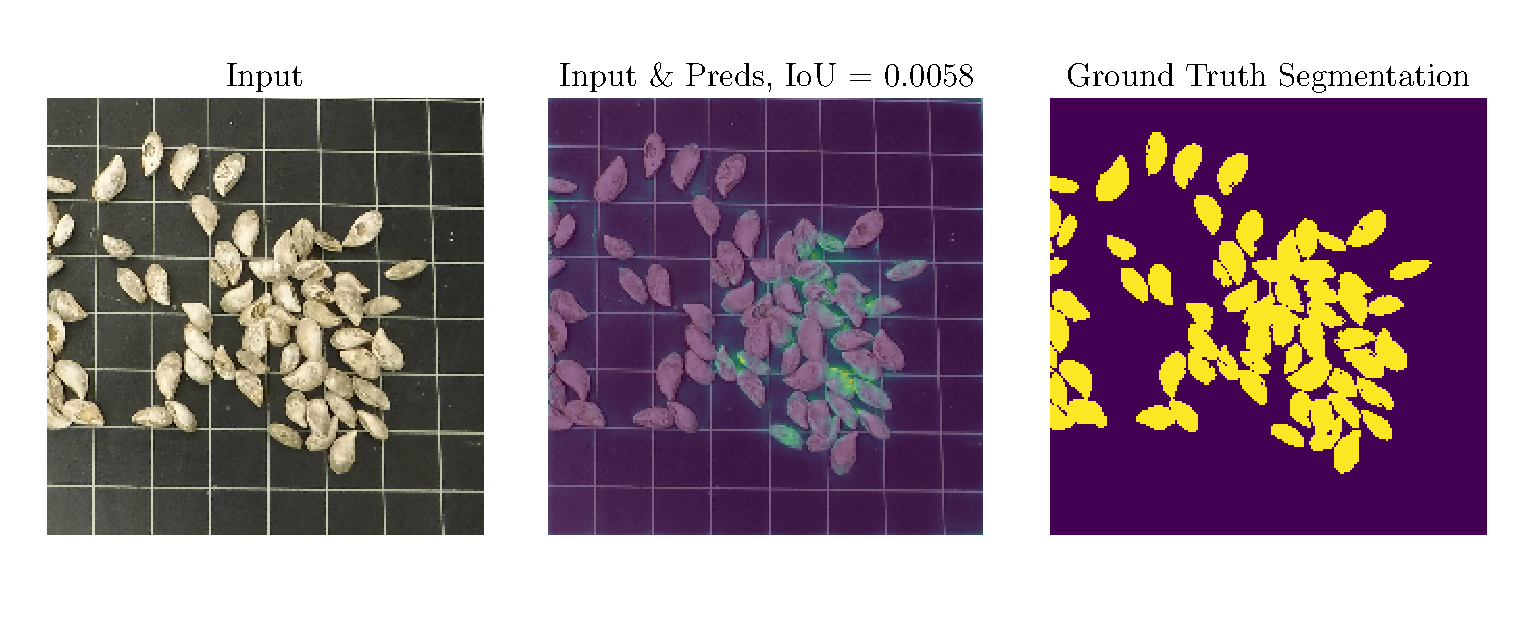
\includegraphics[width=0.9\linewidth]{\zshot/val_101-lab_100__Lab_3796-1_2018-08-13_image-1_patch_width1200__fcn8s_lr1e-03_wd5e-04_bs25_ep80_seed4_epoch70.eps}}
\subfigure{
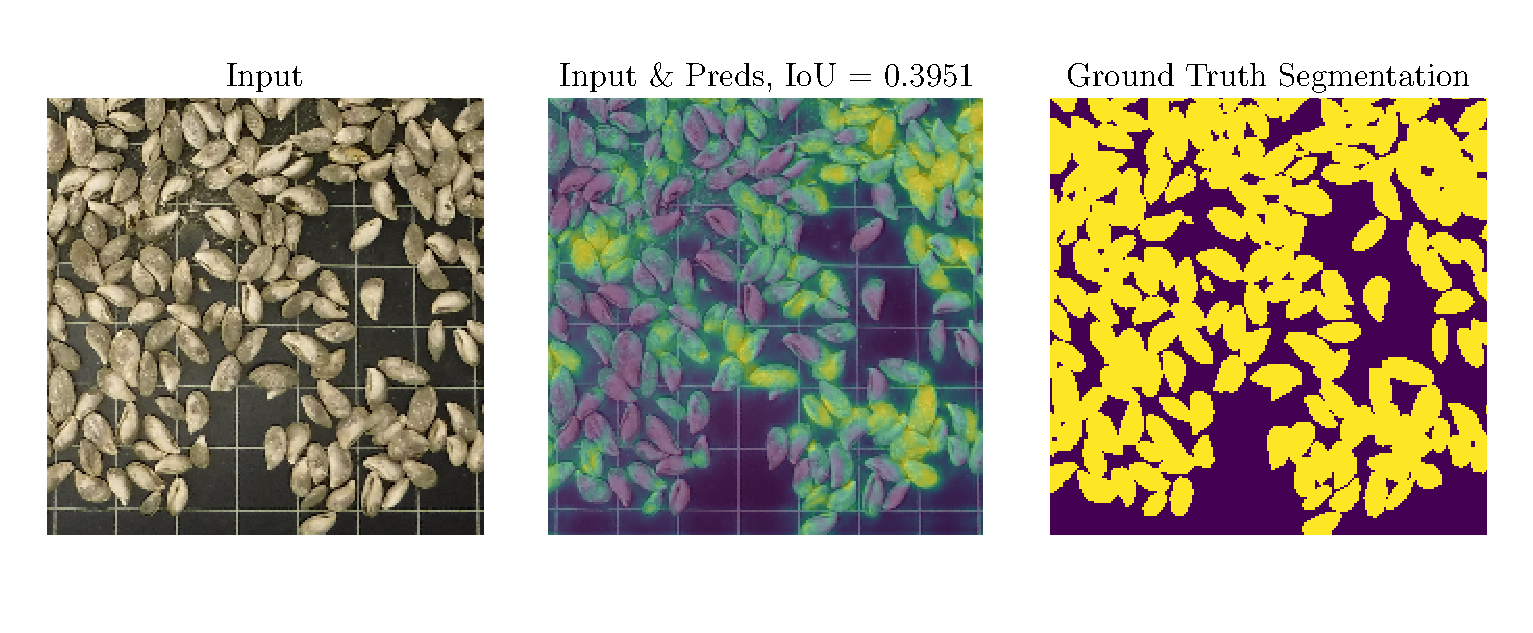
\includegraphics[width=0.9\linewidth]{\zshot/val_101-lab_100__Lab_3798-2_2018-08-13_image-1_patch_width1200__fcn8s_lr1e-03_wd5e-04_bs25_ep80_seed4_epoch70.eps}}
\subfigure{
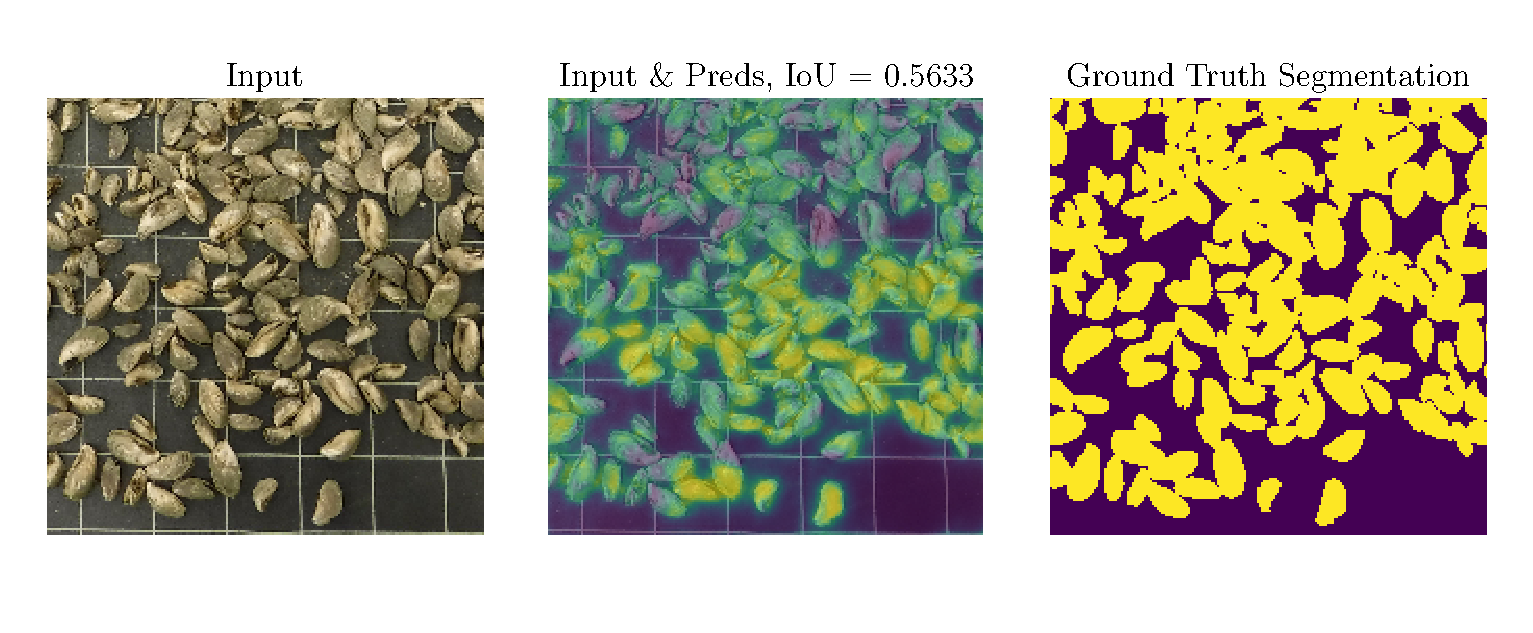
\includegraphics[width=0.9\linewidth]{\zshot/val_101-lab_100__Lab_3801-1_2018-07-11_image-1_patch_width1200__fcn8s_lr1e-03_wd5e-04_bs25_ep80_seed4_epoch70.eps}}

\caption{Qualitative results and intersection-over-union (IoU) score arising
from training the~\texttt{FCN8s} model on~\emph{in-situ} underwater data
(\texttt{val\_v101} split) and testing on Lab data (\texttt{v100}) zero-shot. 
The first column is an input patch in RGB format, second column 
overlays the real valued sigmoid prediction score with the input, and the last 
row are the ground truth binary masks. A failure case is shown in the first
row, and more successful cases in other rows. See text for more details. 
Note: predictions are binarized for calculating IoU. All images are $1200$
square pixels for clarity.}
\label{fig:zero-shot-situ-lab}
\end{figure}


\subsection{Predicting Live Mussel Count}

The labels in the lab analysis for all $N=40$ images from the 2019 Lab test 
split were used to characterize the irreducible error between 
the~\texttt{Count} and~\texttt{Biomass} variables. This serves as a key
baseline before attempting to predict live mussel count using DL. 
Figure~\ref{fig:count-from-biomass} depicts this relationship before and after 
correcting biomass by the mussel size distribution variable. 

For sample index $i$, a size distribution vector $\gamma \in \mathbb{R}^8$ with 
elements $j$ being the fraction of mussels not passing the $X_j$ mm sieve, 
$X \in \{16, 14, 12.5, 10, 8, 6.3, 4, 2\}$, the biomass $\text{B}_i$ was 
adjusted according to:

\begin{equation} \label{eq:size-distribution}
\text{Count}_i = \text{B}_i \cdot \Sigma_{j=1}^8 \bigg( \gamma_j \cdot  
\sqrt{\frac{2 \text{mm}}{X_j}} \bigg)
\end{equation}

The constant 2 mm in the numerator of Eq.~\eqref{eq:size-distribution} is the 
minimum sieve size, such that biomass associated with this bin contributes 
$1:1$ to the mussel Count, while the weight associated with biomass belonging 
to larger mussels decreases with the square root of the ratio of the diameter
to the smallest 2 mm diameter.

\begin{figure}
\centering
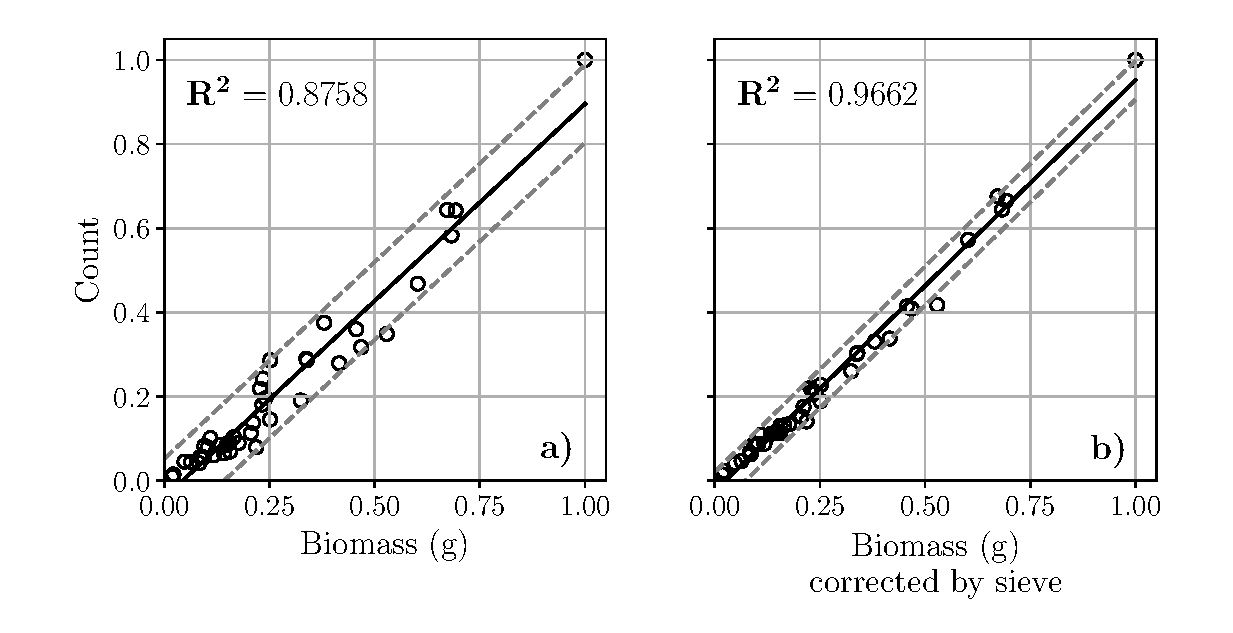
\includegraphics[width=0.9\linewidth]{img/lab_count_from_biomass.eps}
\caption{The relationship between live mussel count and biomass (grams)
for all $N=40$ samples from the 2019~\texttt{Lab} dataset, (a) before, and (b) 
after correcting for the size distribution using
Eq.~\eqref{eq:size-distribution}. The dashed lines indicate two standard
deviations from the line of best fit.}
\label{fig:count-from-biomass}
\end{figure}

\section{Conclusion}

\clearpage

%\bibliographystyle{spbasic} % basic style, author-year citations
\bibliography{CCIW_Zebra}   % name your BibTeX data base

\clearpage

\appendix

\section{Data Annotation Services}

\begin{table}[]
\centering
\caption{A comparison of three image labeling services for generating ground
truth semantic segmentation masks for mussel images:
\texttt{LabelMe}~(\url{https://github.com/wkentaro/labelme}),
\texttt{Figure Eight}~(\url{https://figure-eight.com/}),
and~\texttt{Scale AI}~(\url{https://scale.com/}).
Analysis done assuming two ($C=2$) classes ``mussel'' and ``background'', but
is expected to remain consistent for $C \leq 20$. Row F) ``Latency'' means the
time elapsed between when a label is requested for a particular image and the
time it is delivered, whereas G) ``Throughput'' refers to the number of images
processed per unit time (parallelism, i.e., many workers, increases
throughput). Note: The asterisk ($^*$) for J) for~\texttt{Figure Eight} means
that the user is responsible for the creation of test examples that
automatically reject low quality judgments, otherwise the user must manually
reject them. Rejected judgments incur the same fee as accepted judgments.}
\begin{tabular}{lccc}
\toprule
Service & Manual (\texttt{LabelMe}) & \texttt{Figure Eight} & \texttt{Scale AI} 
\\ \midrule
A) Interface type & Desktop GUI & Web Interface & API Only \\ \midrule
B) Initial setup complexity \\ (Amazon MTurk = 10) & 2 & 5 & 1 \\ \midrule
C) Length of trial \\ (images labeled) & NA & 1000 (Paid) & 5 (Free) \\ \midrule
D) Minimum fee after trial & NA & 10,000 USD & NA \\ \midrule
E) Cost per image (USD) & NA & 2.25 & 6.40 \\ \midrule
F) Latency (minutes) & $1-10$ & $< 60$ & $60-240$ \\ \midrule
G) Throughput & Low & High & Medium \\ \midrule
H) Quality & High & Medium & High \\ \midrule
I) Guaranteed label for \\ all pixels & No & No & Yes \\ \midrule
J) User responsible for \\ quality assurance (QA) & Yes & Yes$^*$ & No \\  
\midrule
K) Ability to edit \\ labels in~\texttt{LabelMe} & Yes & Yes & No \\ \midrule
L) User support & Github & Email & Slack \\ 
\bottomrule
\end{tabular}
\end{table}

\subsection{Figure Eight}

Additional settings were required for good results with this platform. 
Under the Design tab, at the bottom of the page there is an option to enable 
the Code Editor. A new field ``CML'' appears in the editor, which was modified 
as follows:

\begin{lstlisting}[language=html, frame=single]
<cml:shapes label="Draw Shapes" name="annotation" 
type="['polygon']" image-url="{{image_url}}" 
polygon-threshold="0.15" class-threshold="0.1" 
ontology="true" crosshair="false" validates="required" 
class-agg="cagg_0.1" polygon-agg="0.1" gold="true"/>
\end{lstlisting}

The variables modified were: 

\begin{description}
\item[polygon-threshold] The minimum time it should take a contributor to
complete a page of work. When triggered, the contributor will be removed from
your job. Increased from default of 10 to 20 seconds.
\end{description}

These variables are documented here:\url{ 
https://success.figure-eight.com/hc/en-us/articles/360016693051-Guide-to-Polygon-Job-Design-Test-Questions-and-Aggregation}

Under Settings $>$ Contributors:

Increased the ``contributor level'' from level 1 -- \textbf{Fastest
Throughput}: All qualified contributors, to level 3 -- highest quality: 

Under Settings $>$ Quality Control:

\begin{description}
\item[Minimum Time Per Page] The minimum time it should take a contributor to
complete a page of work. When triggered, the contributor will be removed from
your job. Increased from default of 10 to 20 seconds.

\item[Results] check the box to disable responses to test questions.
\end{description}

Post processing json output from FigureEight for validation in LabelMe. We need 
to convert the report generated by FigureEight, which is in jsonstring format, 
into plain json. 

\begin{lstlisting}[language=bash, frame=single]
sed '1s/^/[/; $!s/$/,/; $s/$/]/' in.json > out.json

1  s/^/[/      # Insert a left bracket at the beginning of the first line
$! s/$/,/      # On all but the last line append a comma
$  s/$/]/      # Append a right bracket to the last line
\end{lstlisting}

\subsection{Scale AI}

This section enumerates the complete set of steps to process the output of the 
Scale AI platform for use by the python model training scripts.

\begin{enumerate}
\item Run the python
notebook~\href{https://github.com/AngusG/cciw-zebra-mussel/blob/master/labelme/scale}{postprocess-scale-labels.ipynb}
to convert the RGB colour labels from the~\texttt{Scale AI} API into the format
consistent with the~\texttt{labels.txt} file used by~\texttt{LabelMe}.

\item Run the python
notebook~\href{https://github.com/AngusG/cciw-zebra-mussel/blob/master/labelme/voc-images-and-masks-to-patch.ipynb}{voc-images-and-masks-to-patch.ipynb}
to extract small patches from each labeled image and mask for training and
validation.

\item Populate the test.txt file for VOC format:

\begin{lstlisting}[language=bash, frame=single]
user@ws1:~/Dataset/Test/GLNI/port/scale/patches$ 
ls -l *.png >> VOCdevkit/VOC2012/ImageSets/Segmentation/test.txt
\end{lstlisting}

\item Copy masks into the relevant VOCdevkit folder:

\begin{lstlisting}[language=bash, frame=single]
user@ws1:~/Dataset/Test/GLNI/port/scale/patches$ 
cp -av *.png VOCdevkit/VOC2012/SegmentationClass/
\end{lstlisting}

\item Copy jpeg images into the relevant VOCdevkit folder:

\begin{lstlisting}[language=bash, frame=single]
user@ws1:~/Dataset/Test/GLNI/port/scale/patches$ 
cp -av *.jpg VOCdevkit/VOC2012/JPEGImages/
\end{lstlisting}

\item Confirm that each folder contains the same number of images:
\begin{lstlisting}[language=bash, frame=single]
ls -l VOCdevkit/VOC2012/SegmentationClass | wc -l
ls -l VOCdevkit/VOC2012/JPEGImages/ | wc -l
\end{lstlisting}

\end{enumerate}

\subsection{Editing Segmentation Masks in GIMP}

This section outlines a procedure for editing segmentations masks that are 
already in PNG format, for example to clean up the automatically generated 
masks for the Lab images from the
notebook~\href{https://github.com/AngusG/cciw-zebra-mussel/blob/master/labelme/autolabel-lab-testing-set.ipynb}{autolabel-lab-testing-set.ipynb}.

I recommend using the~\href{https://www.gimp.org/}{GNU Image Manipulation
Program} (GIMP), which is a free and open source professional graphics program.

\begin{enumerate}
\item Select a~\texttt{*.jpg} image, right click and open with GIMP Image 
Editor.
\item In the Layers pane, select this jpg layer and click on the paint brush 
icon ``Lock pixels'' to freeze this layer.
\item From the main menu, select File, Open as Layers..., and select the PNG 
mask associated for the image.
\item Select the PNG mask from the layers pane and change the Opacity value
from $100\%$ to $50\%$.

\item To efficiently label data, I made use of the ``Free Select Tool'' from
the Toolbox, which can be enabled with the keyboard shortcut ``f''. I then fill
in the polygon drawn with the Free Select Tool using the ``Bucket Fill Tool''. 
The Bucket Fill tool default shortcut is ``Shift B'', which can be cumbersome 
when switching rapidly back and fourth. I created a new shortcut ``b'' using 
the instructions 
here:~\url{https://docs.gimp.org/2.10/en/gimp-concepts-shortcuts.html}.

\item Change the foreground color to solid red (\texttt{\#ff0000}), consistent
with the existing indexed colormap of the mussel labels, but a bit brighter to
make it easier to see which pixels have been changed in GIMP. The
notebook~\texttt{run-crf-on-gimp-masks.ipynb} ultimately merges the two red
variants into a single ``mussel'' label. Change the background color to 
black (\texttt{\#000000}). We will use this to remove any ``false positives'', 
that is, pixels predicted as mussel that should be background.

\item Under Bucket Fill, Tool Options, change ``Affected Area'' to ``Fill whole 
selection''.

\item Use the shorcut ``f'' to enable the Free Select Tool and draw the first 
polygon around a mussel. Note that you may either click to place individual
vertices, or press and hold the left mouse to draw a continous curve. Next, use
the ``b'' or ``Shift+B'' shortcut to switch to Bucket Fill. Ensure ``FG color
fill'' is selected which will use the red colour set previously for mussel. 
Similarly, to label background pixels, switch the Fill Type to ``BG color 
fill''. Repeat this step as necessary until satisfied.

\begin{figure}
\centering
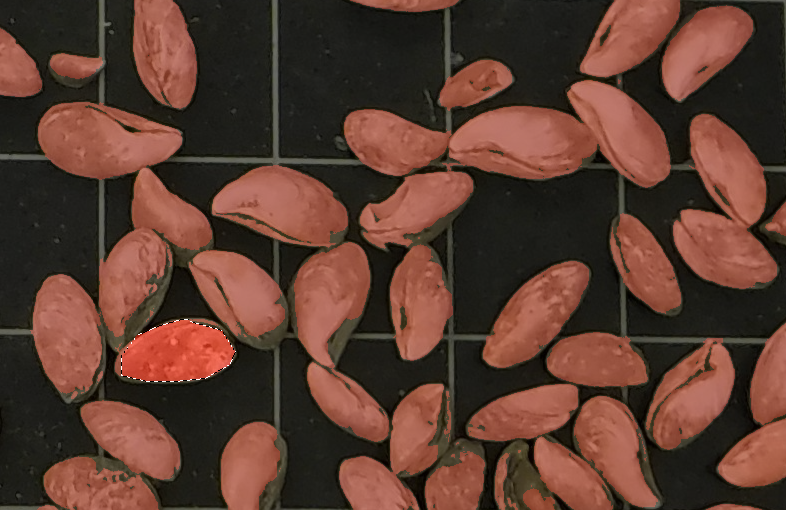
\includegraphics[width=0.4\linewidth]{img/GIMP_edit_mask}
\caption{Modifying mussel segmentation masks using GIMP software. Transparent 
red colour corresponds to mussel label. Selected area corresponds to modified 
label.}
\label{fig:gimp-label}
\end{figure}

\item To export a new mask in the correct format, we will now delete the JPEG 
layer. From the Layers pane, right click on the jpg file and select ``Delete
Layer''. Now select the PNG layer that we have been editing, and restore the 
Opacity to $100\%$. 

\item Select Image $\rightarrow$ Mode $\rightarrow$ Indexed from the 
main menu to change the image from RGB format to indexed color 
format. The default setting, choose optimal colormap can be 
used. For more information 
see~\url{https://docs.gimp.org/2.8/en/gimp-image-convert-indexed.html}.

\item Finally, from the File menu, Export As and append~\texttt{\_gimp.png} to 
the end of the file for reproducibility. Each Lab sample should now be 
associated with the following collection of five (5) images:

\begin{figure}
\centering
\subfigure[]{
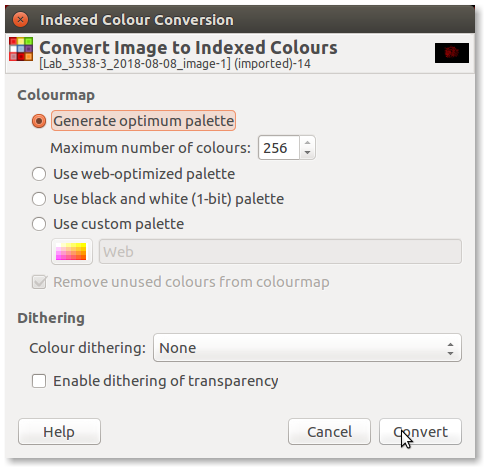
\includegraphics[width=0.4\linewidth]{img/GIMP_Indexed-color-conversion}}
\subfigure[]{
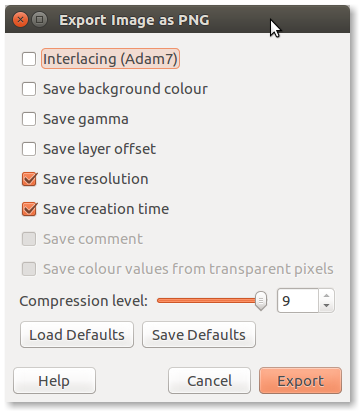
\includegraphics[width=0.34\linewidth]{img/GIMP_Export-Image-as-PNG}}
\caption{gimp-usage}
\label{fig:gimp-export-menu}
\end{figure}

\begin{enumerate}
\item \texttt{Lab\_2907-3\_2018-07-09\_image-1.jpg} -- Original RGB JPEG image.
\item \texttt{Lab\_2907-3\_2018-07-09\_image-1\_mask\_crf.png} -- Indexed color 
PNG mask, noisy output from~\texttt{autolabel-lab-testing-set.ipynb}.
\item \texttt{Lab\_2907-3\_2018-07-09\_image-1\_mask\_crf.xcf} -- GIMP version 
of file (b) for editing.
\item \texttt{Lab\_2907-3\_2018-07-09\_image-1\_mask\_crf\_gimp.png} -- Updated 
indexed color PNG mask after processing in GIMP. Contains two shades of red, 
GIMP changes in bright red.
\item \texttt{Lab\_2907-3\_2018-07-09\_image-1\_mask\_crf\_gimp\_crf.png} -- 
After processing of file (d) with~\texttt{run-crf-on-gimp-masks.ipynb}. Contains
only a single label index, suitable for use with Python DL model training and
testing scripts.

\end{enumerate}

\end{enumerate}

\end{document}
